This section specifies the software architecture requirements and the software
architecture design for web application framework.

\subsection{Architecture Requirements}
The web application framework provides the software architecture for the software
providing browser based access to human users.

\subsubsection{Access and Integration Requirements}
The web application must be usable by humans using any standards compliant web
browser. The system should be usable by the latest versions of the Mozilla 
Firefox, Chrome, Safari, Opera and Internet Explorer. The web
application will need to integrate with the services/business processes layer
via a REST API.

\subsubsection{Quality Requirements}
The most important quality requirements for the web application layer are
\begin{itemize}
	\item Usability
	\item Maintainability
	\item Flexibility
	\item Performance
\end{itemize}
	
\subsubsection{Architectural Responsibilities}
The architectural responsibilities of the Web Application Framework are shown in 
Figure \ref{fig:webApplicationFrameworkResponsibilities}
\begin{figure}[H]
	\begin{center}
	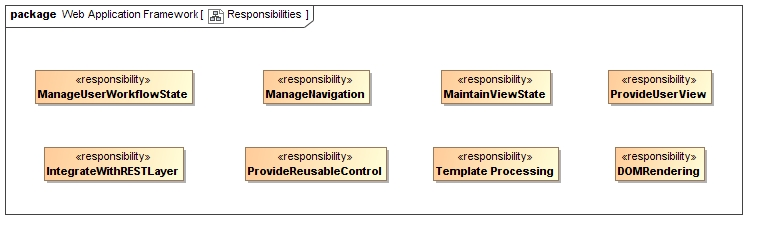
\includegraphics[scale=0.35]{../Diagrams and Charts/Web Application Framework/Responsibilities.jpg}
	\caption{The architectural responsibilities of the Web Application Framework}
	\label{fig:webApplicationFrameworkResponsibilities}
	\end{center}
\end{figure}

\subsubsection{Architecture Constraints}
The architectural constraints of the system are propagated directly to all 
components including the web application framework. It must hence be open source
and make use of public standards. The chosen technology should also be well 
supported and documented and allow for possible mobile integration.

\subsection{Architecture Design}
This section specifies the very high-level software architecture design, i.e.
the software architecture design for the top level of granularity. Including 
allocation of architectural responsibilities to architectural components, any
tactics which should be used at the current level of granularity to address
quality requirements.

\subsubsection{Tactics}
Tactics which should be used to address the quality requirements should include:
\begin{itemize}
	\item caching of pre-generated and pre-populated HTML pages for performance
	\item virtual DOM for in-memory updates, incremental builds and efficient 
	diffing based on differentiation between static and dynamic DOM elements
\end{itemize}
\subsubsection{Architectural Components}
The architectural components of the  Web Application Framework are shown in Figure \ref{fig:webApplicationFrameworkResponsibilityAllocation}
\begin{figure}[H]
	\begin{center}
	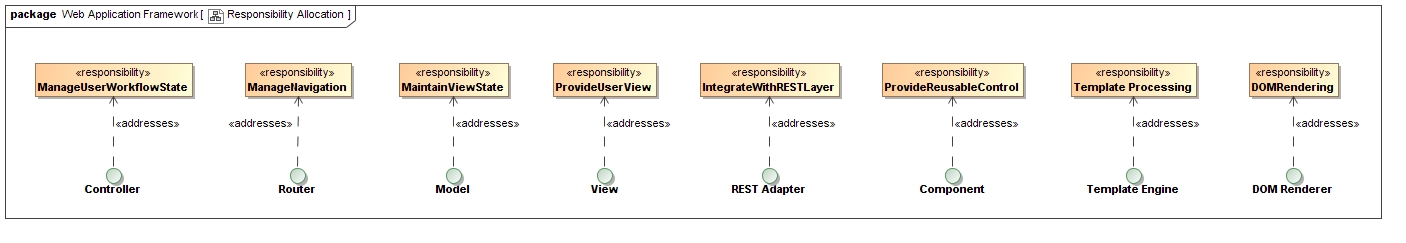
\includegraphics[scale=0.35]{../Diagrams and Charts/Web Application Framework/ResponsibilityAllocation.jpg}
	\caption{The abstract components to which the Web Application Framework responsibilities are assigned.}
	\label{fig:webApplicationFrameworkResponsibilityAllocation}
	\end{center}
\end{figure}

\subsubsection{Frameworks and Technologies}
The web framework will be based on \textbf{ReactJS}. ReactJS is an open-source web
application framework. The framework promises a model in which sub-components
cannot directly affect enclosing components.

Core reasons for using ReactJS:
\begin{itemize}
	\item The framework requires a defined structure which aids in maintainability.
	\item The framework is maintained not only by a community of users but also
	by Facebook and Instagram, this aids further in maintainability due to the 
	constant upkeep of documentation.
	\item The model supports integration with RESTful API services.
	\item Release of React Native which will allow for React based architecture 
	to native Android and iOS applications making the task of developing an 
	application, should time permit, easier.
\end{itemize}
Other frameworks were considered;
\begin{itemize}
	\item \textbf{AngularJS}: which is a powerful extensible framework with good modularization
, however, there is no consistent way to approach application development which may 
lead to difficulty regarding maintenance. The virtual DOM approach in ReactJS is more
efficient. Angular is also being replaced by ReactJS as the current standard for web 
application development and as a team with minimal experience in Angular we decided 
that we'd rather get experience in a future standard which is also easier to learn.
	\item Ember.js
	\item Backbone.js
\end{itemize}

\paragraph{Concrete Realization of Architectural Components}
The concrete realization of components within \textbf{ReactJS} are shown in Figure
\paragraph{Tactics}
\paragraph{Tools}
\begin{itemize}
	\item Uses JavaScript so no need to learn another language/syntax.
\end{itemize}
\paragraph{Concepts and Constraints for Application Components}